\documentclass[12pt,a4paper]{report}\usepackage[spanish]{babel}\usepackage[utf8]{inputenc}\usepackage{graphicx}\usepackage{geometry}\usepackage{xcolor}\usepackage{tikz}\usepackage{pgfplots}\usepackage{booktabs}\usepackage{multicol}\usepackage{hyperref}\usepackage{pgf-pie}

\geometry{margin=2.0cm}

\pgfplotsset{compat=1.16}

\definecolor{color1}{RGB}{42, 157, 143}
\definecolor{color2}{RGB}{233, 196, 106}
\definecolor{color3}{RGB}{244, 162, 97}
\definecolor{color4}{RGB}{231, 111, 81}
\definecolor{alura1}{RGB}{40, 100, 180}
\definecolor{alura2}{RGB}{20, 60, 120}

\hypersetup{
    colorlinks=true,
    linkcolor=blue,
    filecolor=magenta,      
    urlcolor=cyan,
    pdftitle={Informe Análisis Alura Store},
    pdfpagemode=FullScreen,
}

\title{
    \vspace{-1.0cm}
    \begin{tikzpicture}[remember picture, overlay]
        \fill[alura1] (0,0) rectangle (\paperwidth,-3cm);
        \node[text=white, font=\Huge\bfseries, anchor=west] at (1cm,-1.5cm) {Informe de Análisis Estratégico};
    \end{tikzpicture}
    \vspace{3cm}
    \Large{\textbf{Alura Store: Evaluación para Desinversión}}\\
    \vspace{1cm}
}

\author{
    \Large{Francisco Beltrán Toledo}\\
    \normalsize{Ingeniero en Electrónica}
}

\date{\today}

\begin{document}

\maketitle

\begin{abstract}
\noindent Este informe presenta un análisis exhaustivo de las cuatro tiendas de Alura Store con el objetivo de identificar cuál de ellas representa la mejor candidata para vender e invertir en un nuevo negocio. Se han evaluado cinco criterios principales: facturación total, categorías más populares, evaluación de clientes, productos más y menos vendidos, y costos de envío. El análisis incluye visualizaciones gráficas de alto impacto y una recomendación estratégica final basada en una ponderación de los factores clave de desempeño.
\end{abstract}

\tableofcontents

\chapter{Introducción}

El Sr. Juan, propietario de Alura Store, ha solicitado un análisis para determinar cuál de sus cuatro tiendas debería vender para invertir en un nuevo negocio. Este informe presenta los resultados de un análisis de datos exhaustivo para apoyar esta decisión estratégica.

La evaluación se ha realizado considerando cinco aspectos clave:
\begin{enumerate}
    \item Facturación total de cada tienda
    \item Categorías más populares por tienda
    \item Promedio de evaluación de clientes
    \item Productos más y menos vendidos
    \item Costo promedio de envío
\end{enumerate}

Cada uno de estos factores ha sido analizado en detalle y se ha asignado un peso específico en la evaluación final para determinar la tienda que representaría la mejor candidata para vender.

\chapter{Metodología}

\section{Fuentes de Datos}
Los datos analizados provienen de los registros de ventas de las cuatro tiendas de Alura Store. Cada tienda cuenta con un conjunto de datos que incluye información sobre productos, categorías, precios, evaluaciones de clientes, costos de envío y ubicación geográfica.

\section{Enfoque Analítico}
Para realizar un análisis justo y objetivo, se han normalizado todas las métricas para permitir una comparación equitativa entre las tiendas. La puntuación total se ha calculado ponderando cada métrica según su importancia relativa:

\begin{itemize}
    \item Facturación total: 35\%
    \item Evaluación de clientes: 25\%
    \item Volumen de ventas: 25\%
    \item Costo de envío: 15\%
\end{itemize}

\section{Herramientas Utilizadas}
El análisis se ha realizado utilizando Python y sus bibliotecas de análisis de datos (Pandas, Matplotlib, Seaborn). Para garantizar la reproducibilidad, todo el código fuente está disponible en el archivo \texttt{analisis\_alurastore.py}.

\chapter{Análisis de Facturación}

\section{Facturación Total por Tienda}

La facturación total es uno de los indicadores más importantes del desempeño financiero de cada tienda. A continuación, se presenta una comparación de la facturación total:

\begin{center}
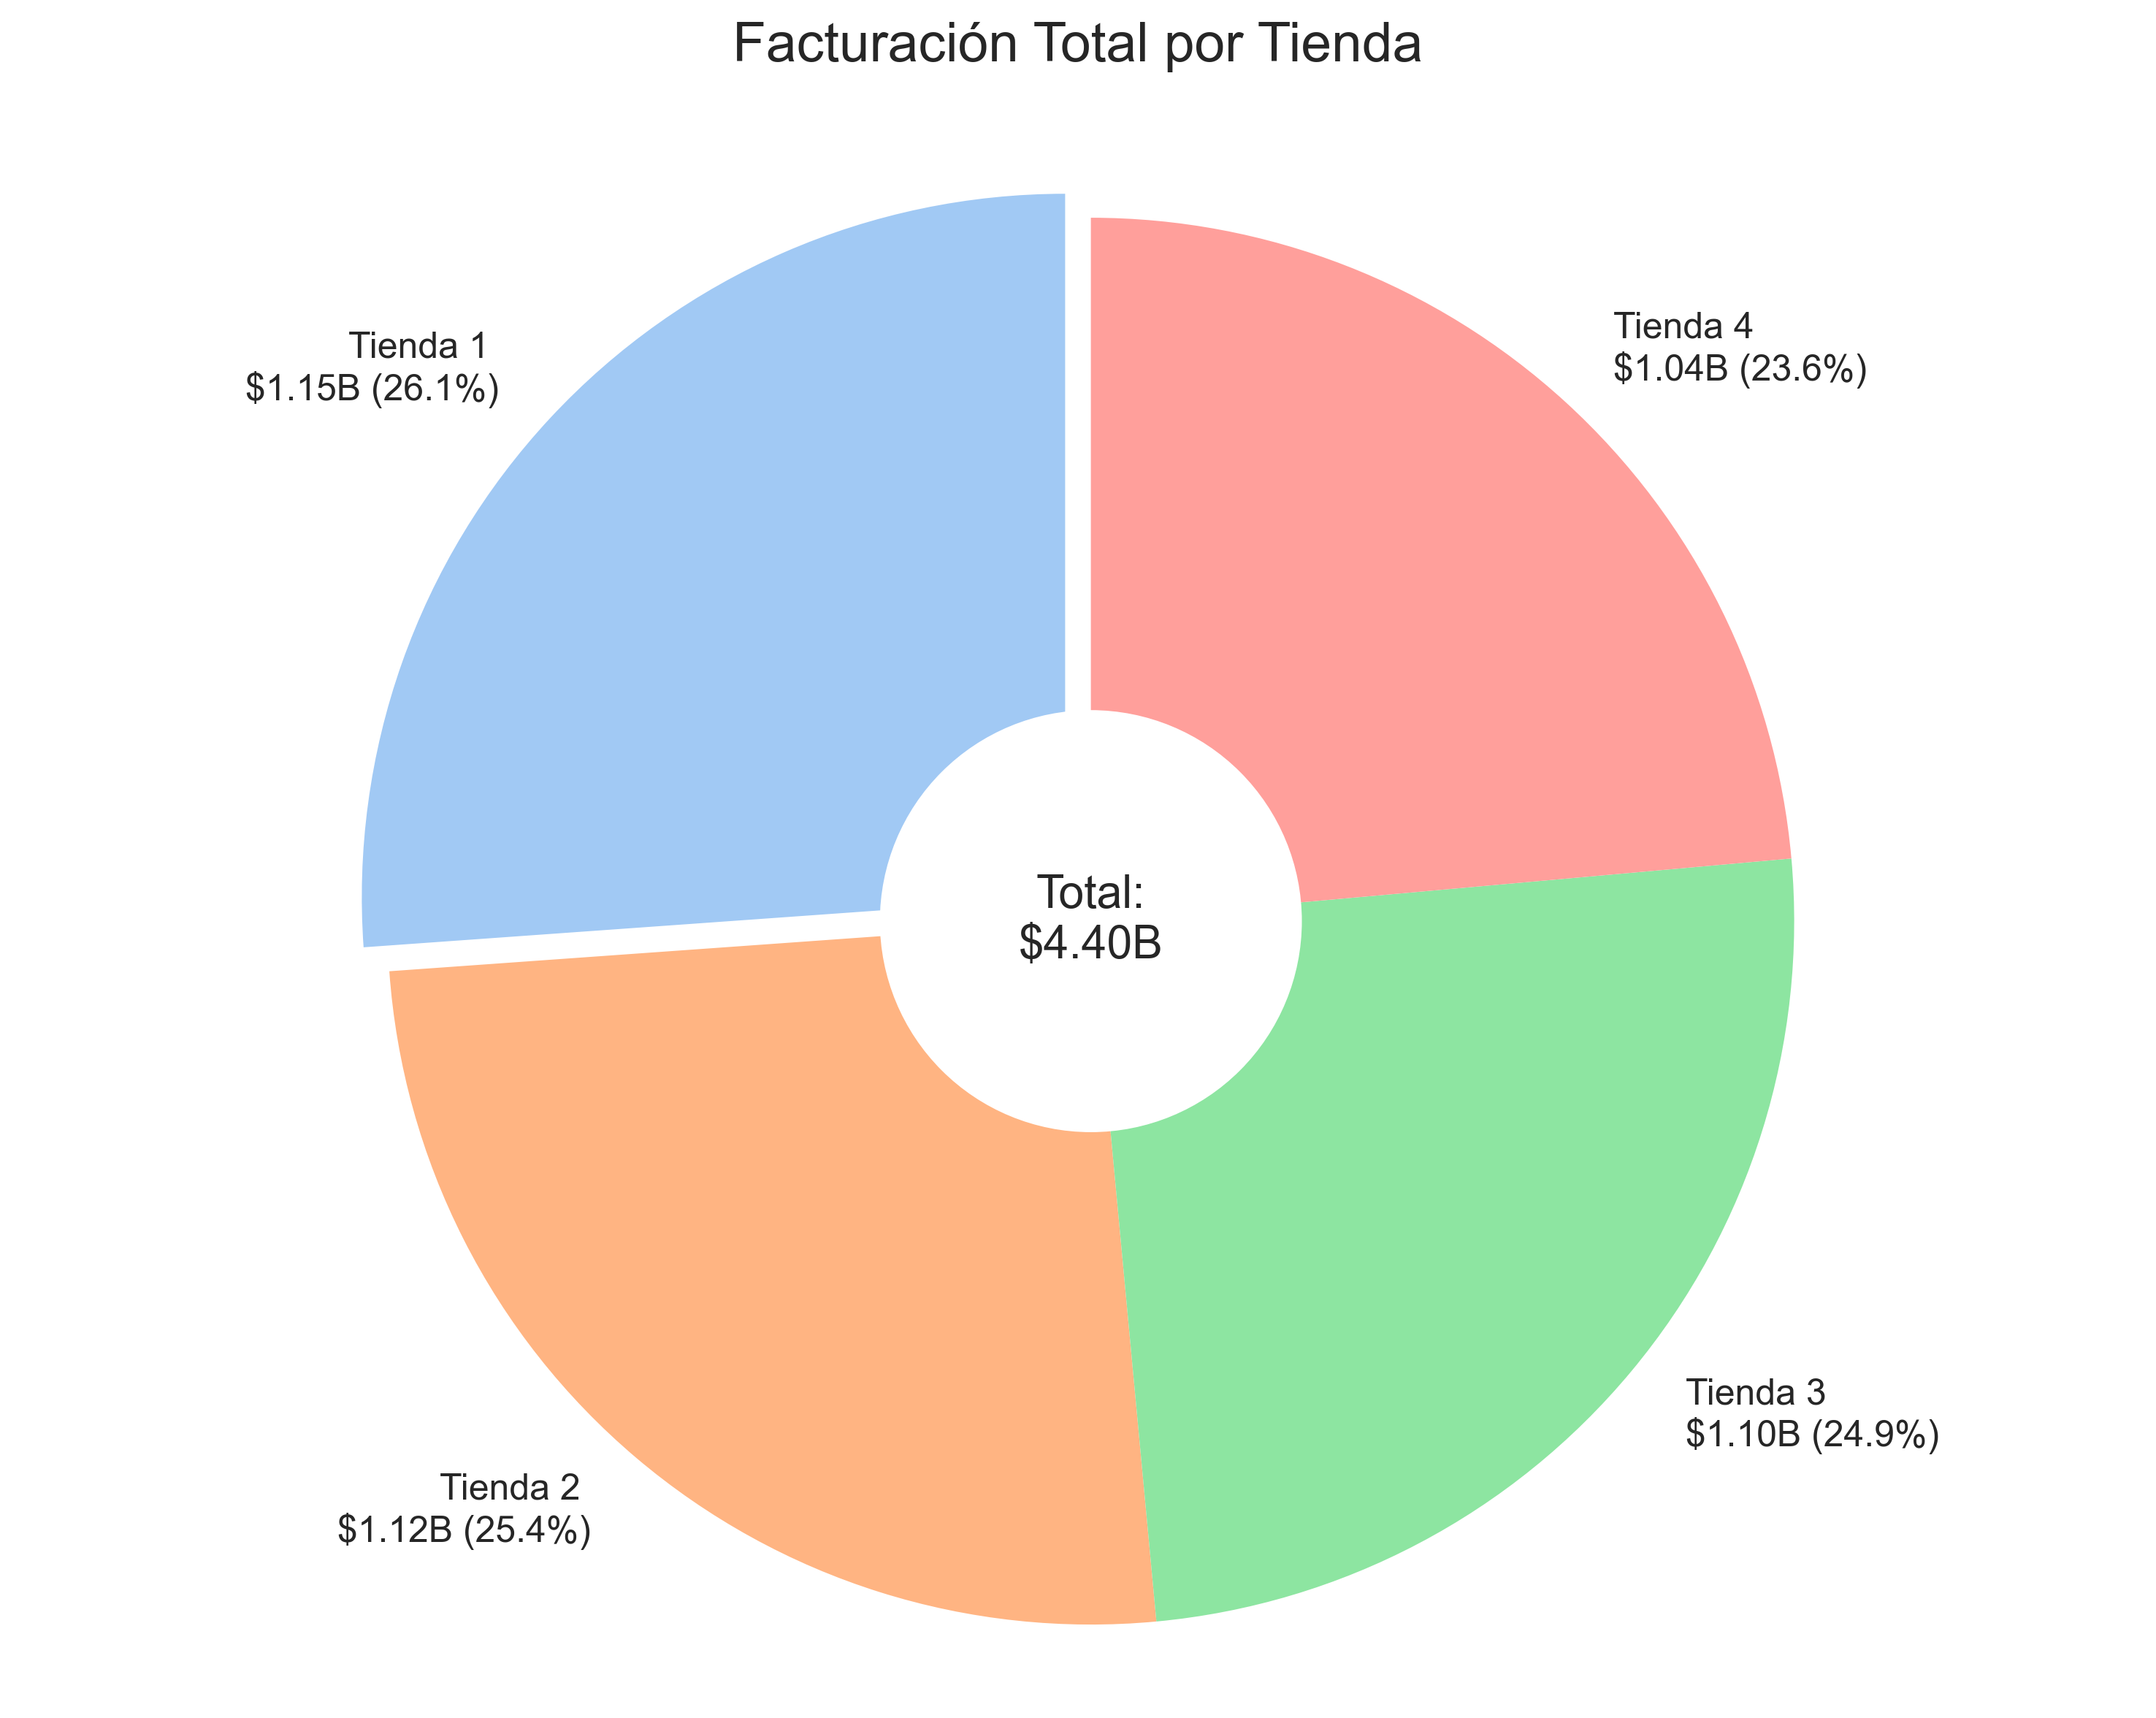
\includegraphics[width=0.9\textwidth]{1_facturacion_total.png}
\end{center}

Como se observa en el gráfico, la Tienda 1 presenta la mayor facturación con \$1,150.9 millones, mientras que la Tienda 4 tiene la menor facturación con \$1,038.4 millones, representando una diferencia de aproximadamente 10\% entre la tienda con mayor y menor facturación.

\chapter{Análisis de Categorías}

\section{Categorías Populares por Tienda}

Un análisis de las categorías más populares revela patrones de consumo importantes en cada tienda:

\begin{center}
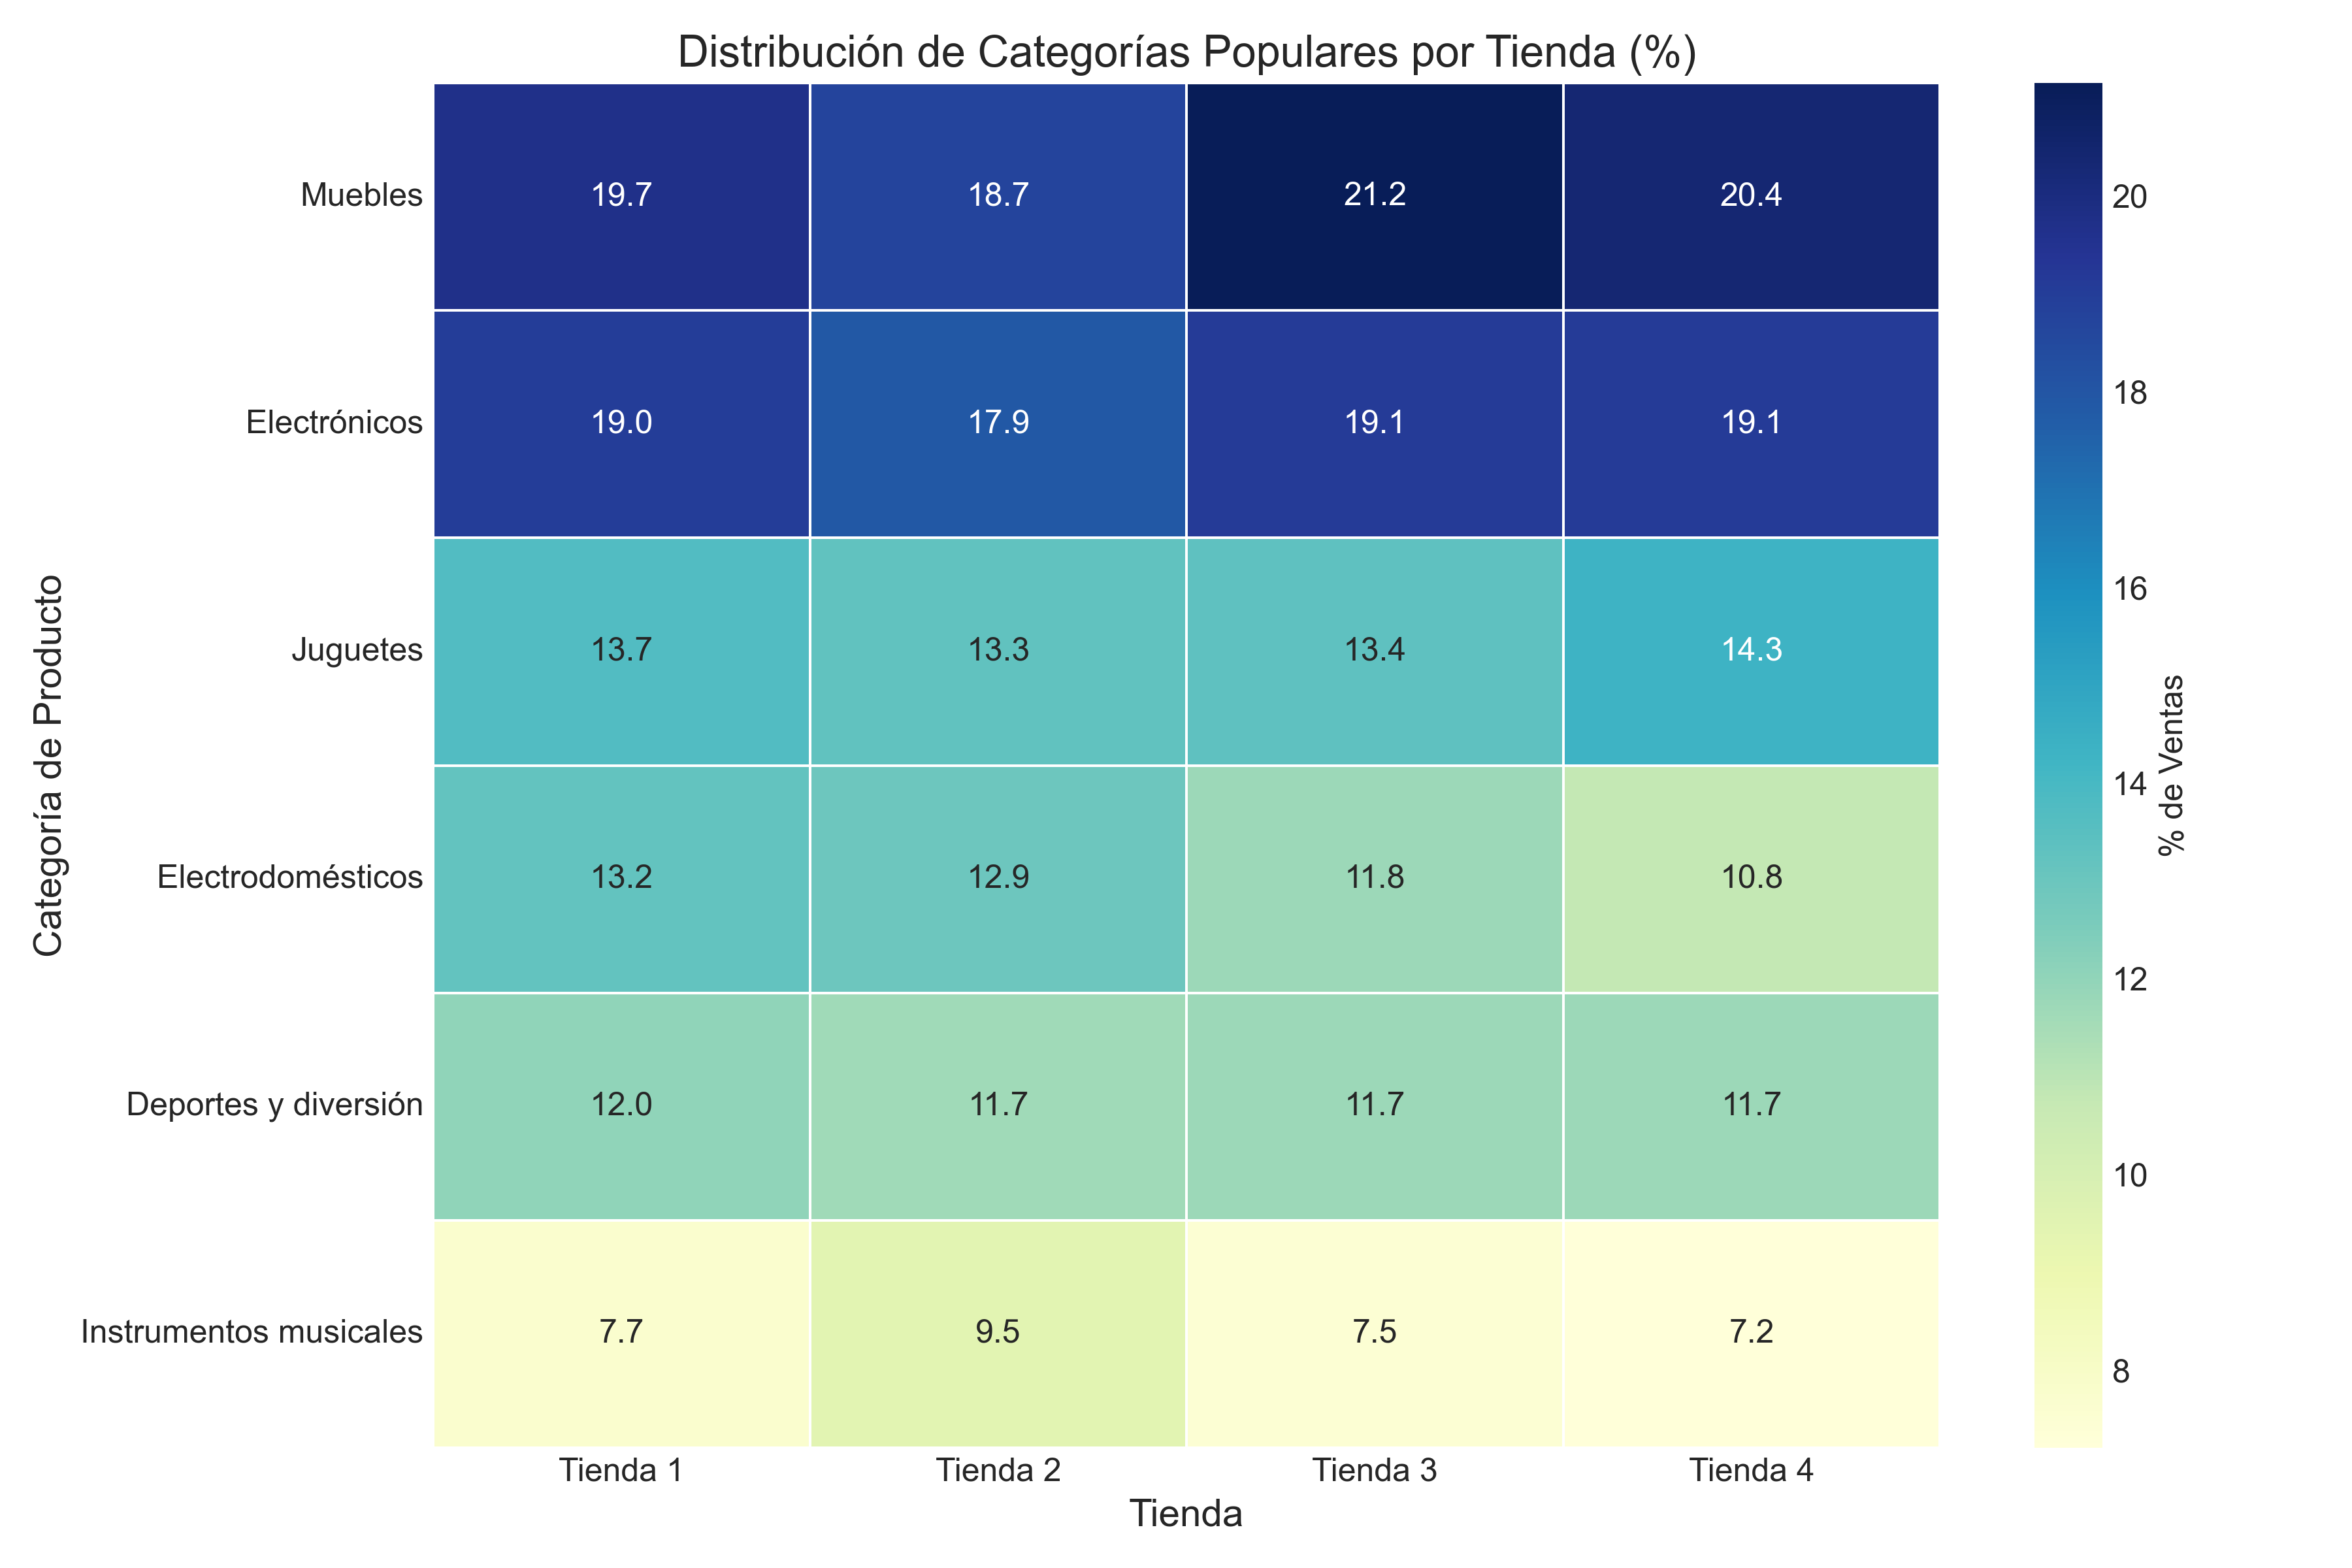
\includegraphics[width=0.9\textwidth]{2_categorias_populares_global.png}
\end{center}

\begin{multicols}{2}
El análisis de las categorías revela que:

\begin{itemize}
    \item \textbf{Muebles} es la categoría más popular en todas las tiendas, representando aproximadamente el 20\% de las ventas.
    \item \textbf{Electrónicos} es la segunda categoría más vendida, con un porcentaje similar en todas las tiendas.
    \item Las categorías de \textbf{Juguetes} y productos para el \textbf{Hogar} muestran un comportamiento consistente entre tiendas.
    \item La categoría \textbf{Otros} (que agrupa categorías menores) representa más de un tercio de las ventas en todas las tiendas.
\end{itemize}

La Tienda 3 muestra la mayor proporción de ventas en Muebles (21.2\%), mientras que la Tienda 2 presenta la menor proporción (18.7\%).

\begin{center}
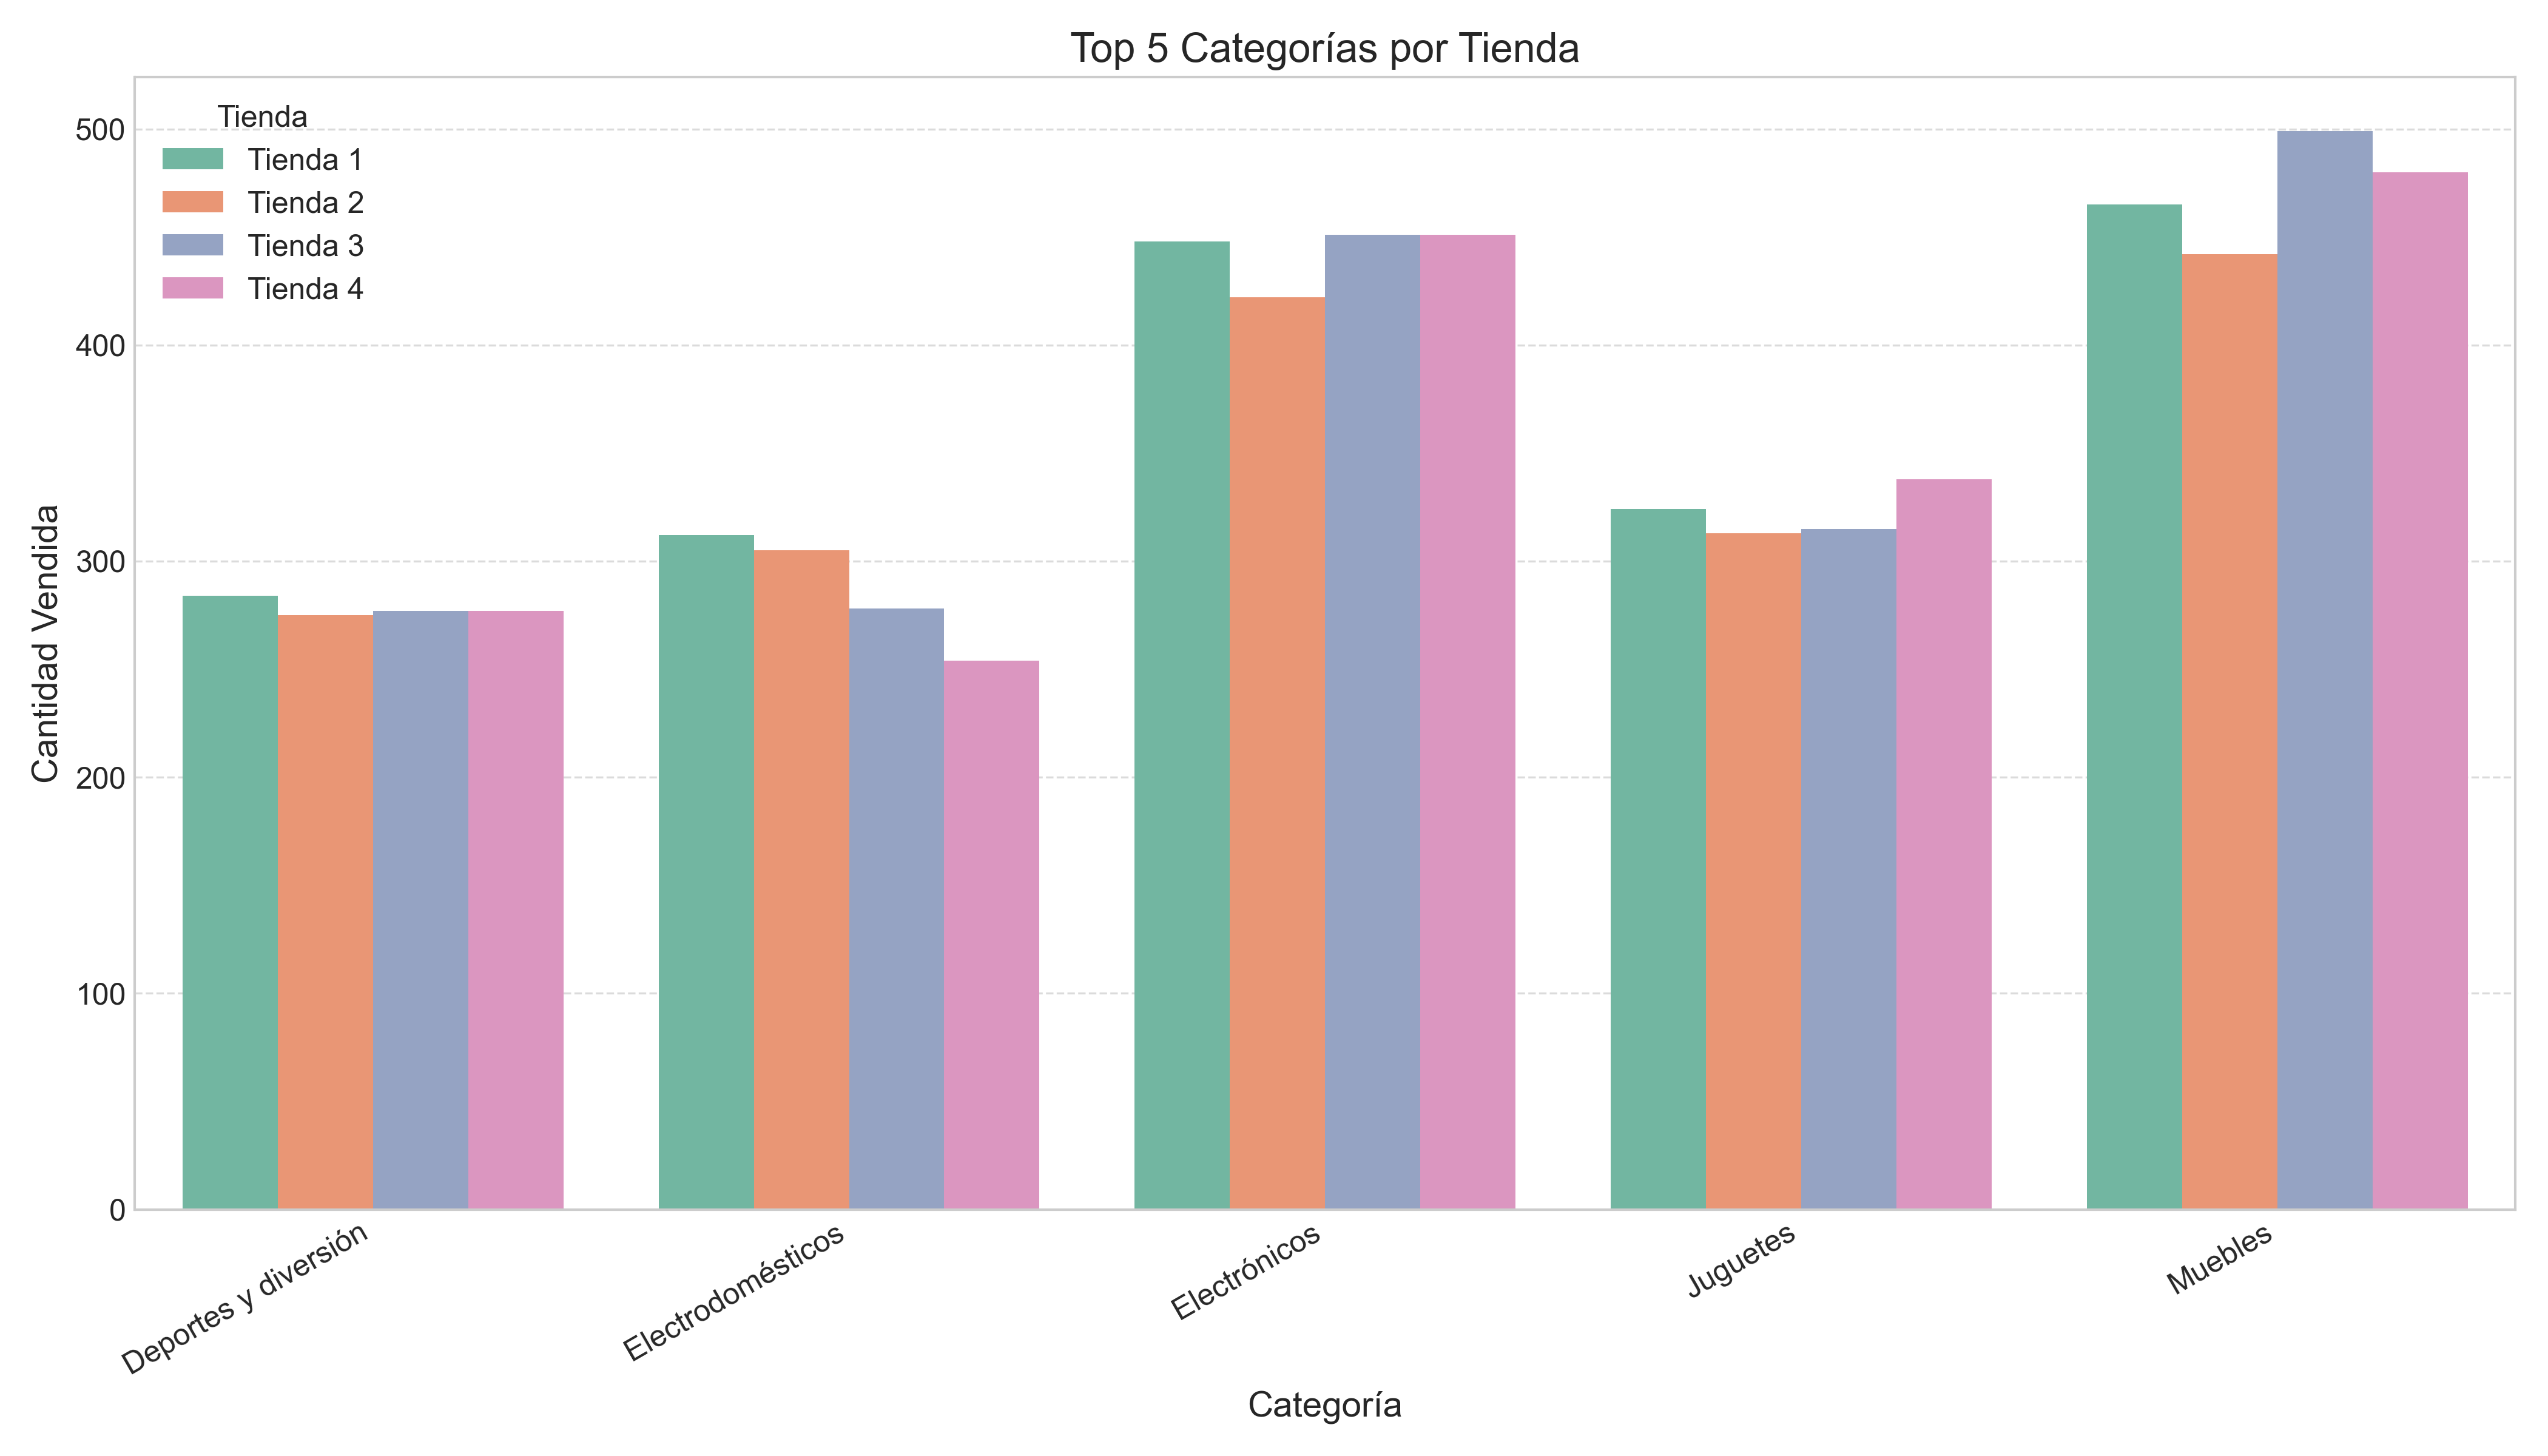
\includegraphics[width=0.95\textwidth]{2_categorias_populares_detalle.png}
\end{center}
\end{multicols}

\chapter{Análisis de Evaluación de Clientes}

\section{Promedio de Evaluación por Tienda}

La satisfacción del cliente es un indicador crucial del éxito a largo plazo. A continuación se presenta el análisis de las evaluaciones promedio:

\begin{center}
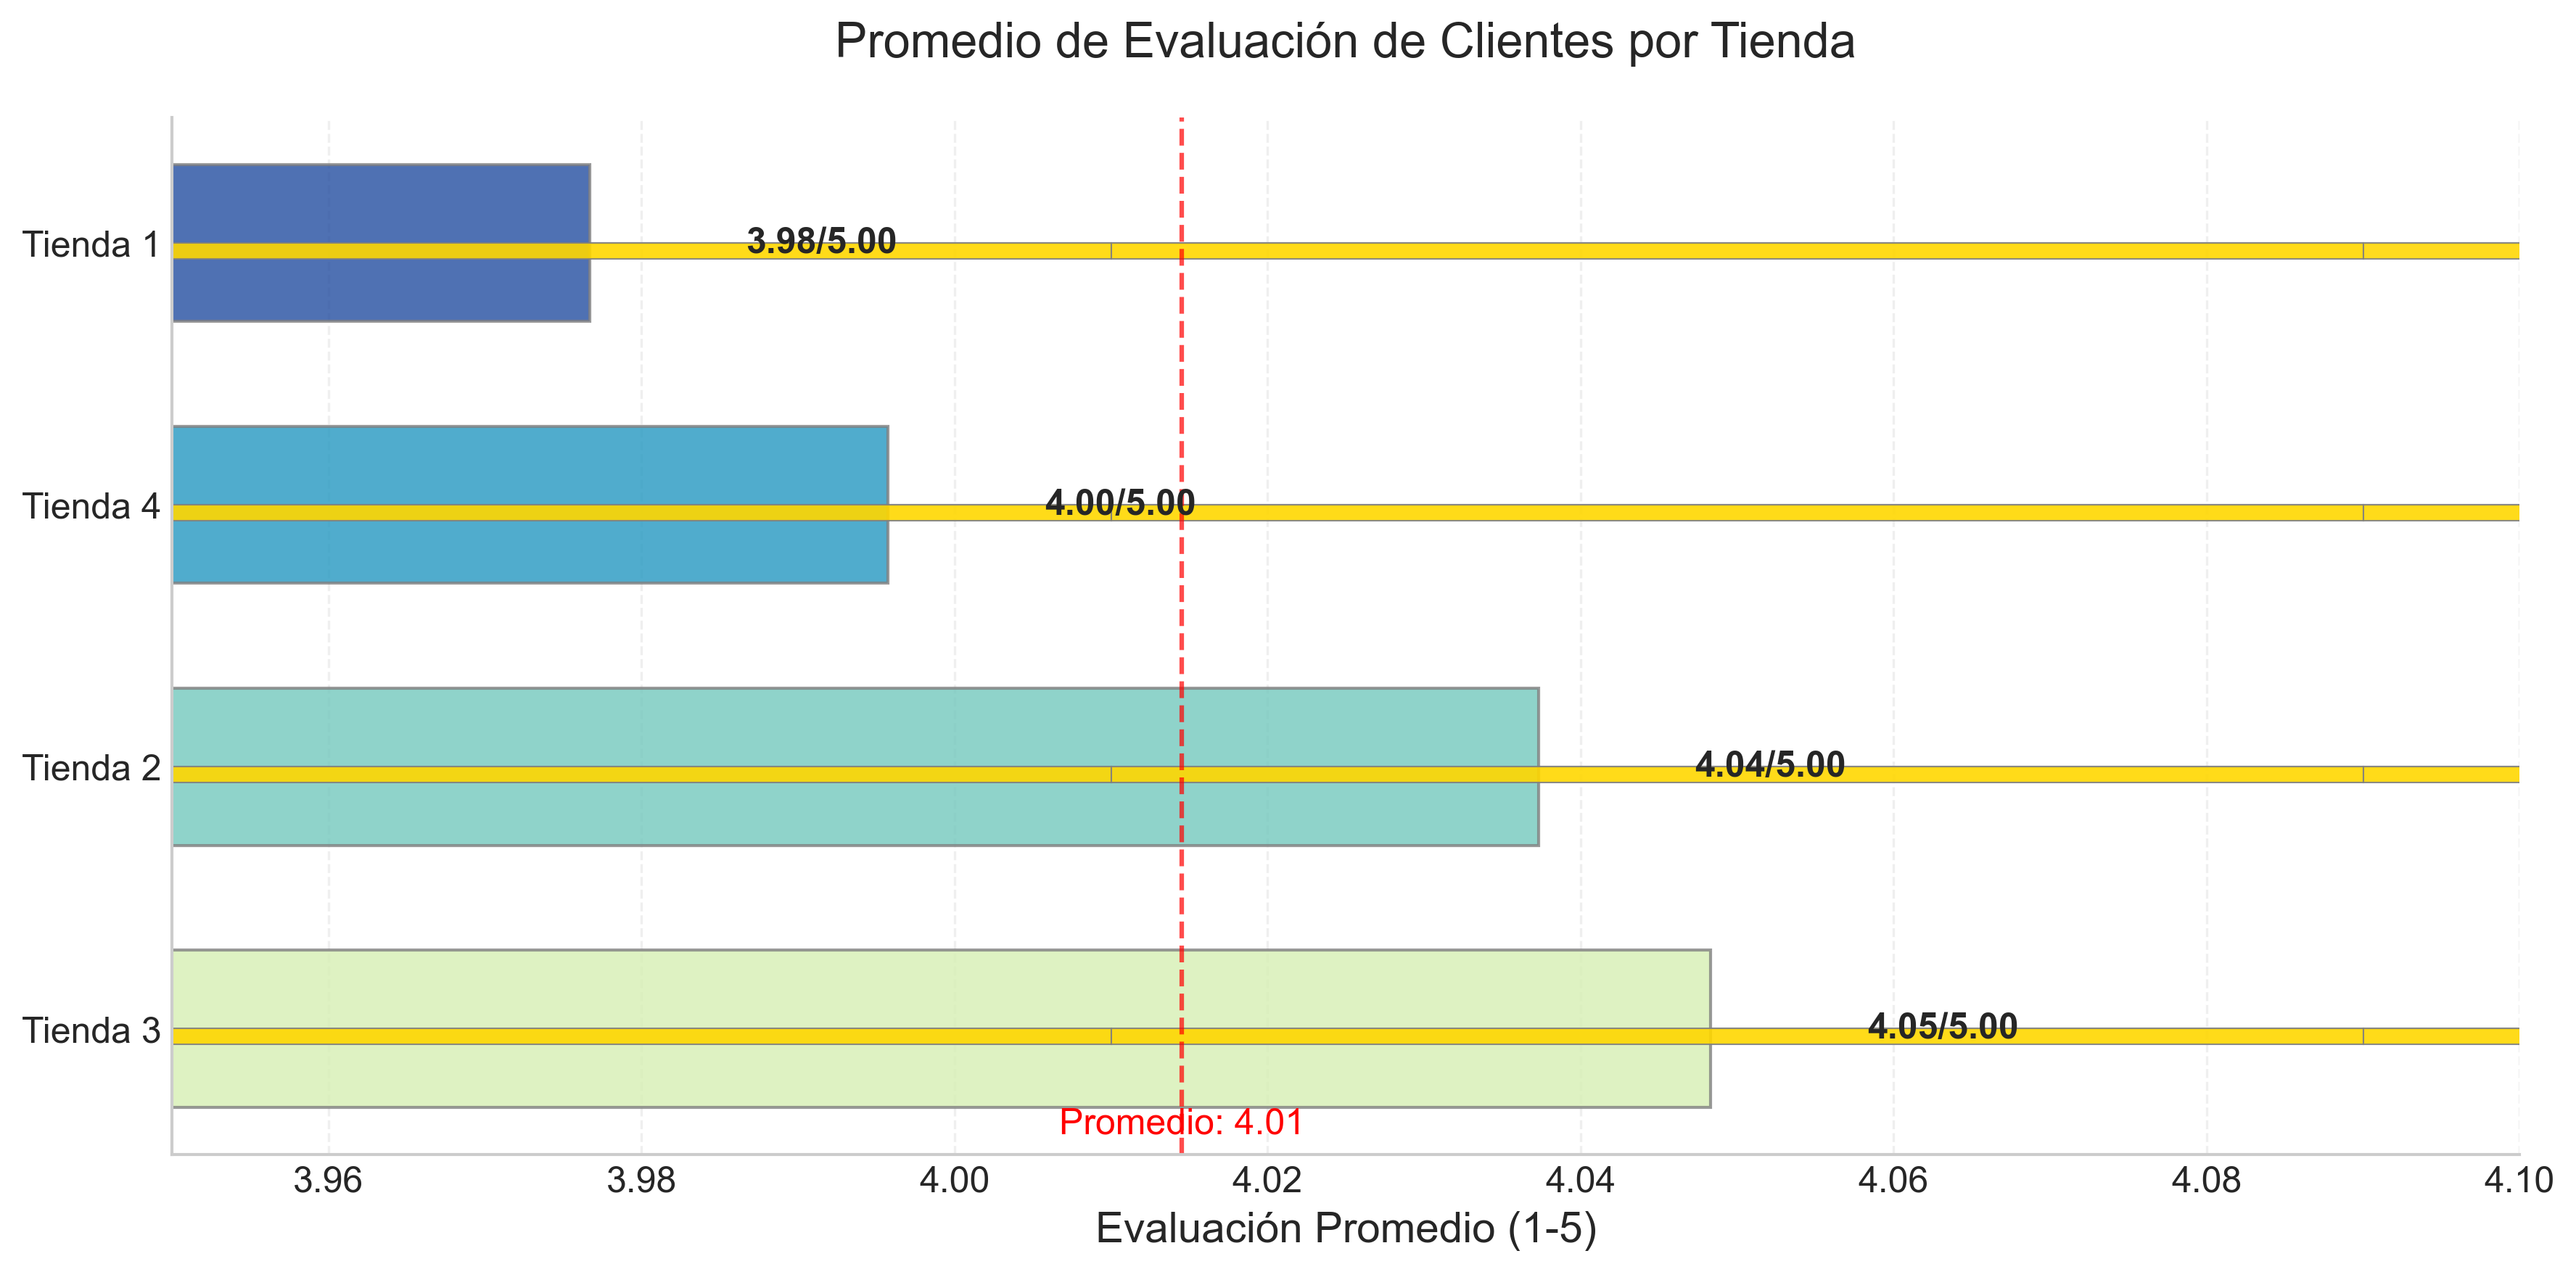
\includegraphics[width=0.9\textwidth]{3_evaluacion_clientes.png}
\end{center}

Los resultados muestran que:

\begin{itemize}
    \item La Tienda 3 tiene la mejor evaluación promedio (4.05 sobre 5).
    \item La Tienda 1 presenta la evaluación más baja (3.98 sobre 5).
    \item En general, todas las tiendas tienen una evaluación satisfactoria, superior a 3.9 sobre 5.
    \item La diferencia entre la tienda mejor valorada y la peor valorada es de apenas 0.07 puntos.
\end{itemize}

\chapter{Análisis de Productos}

\section{Productos Más y Menos Vendidos}

A continuación, se presenta un análisis detallado de los productos más vendidos y menos vendidos por tienda:

\begin{center}
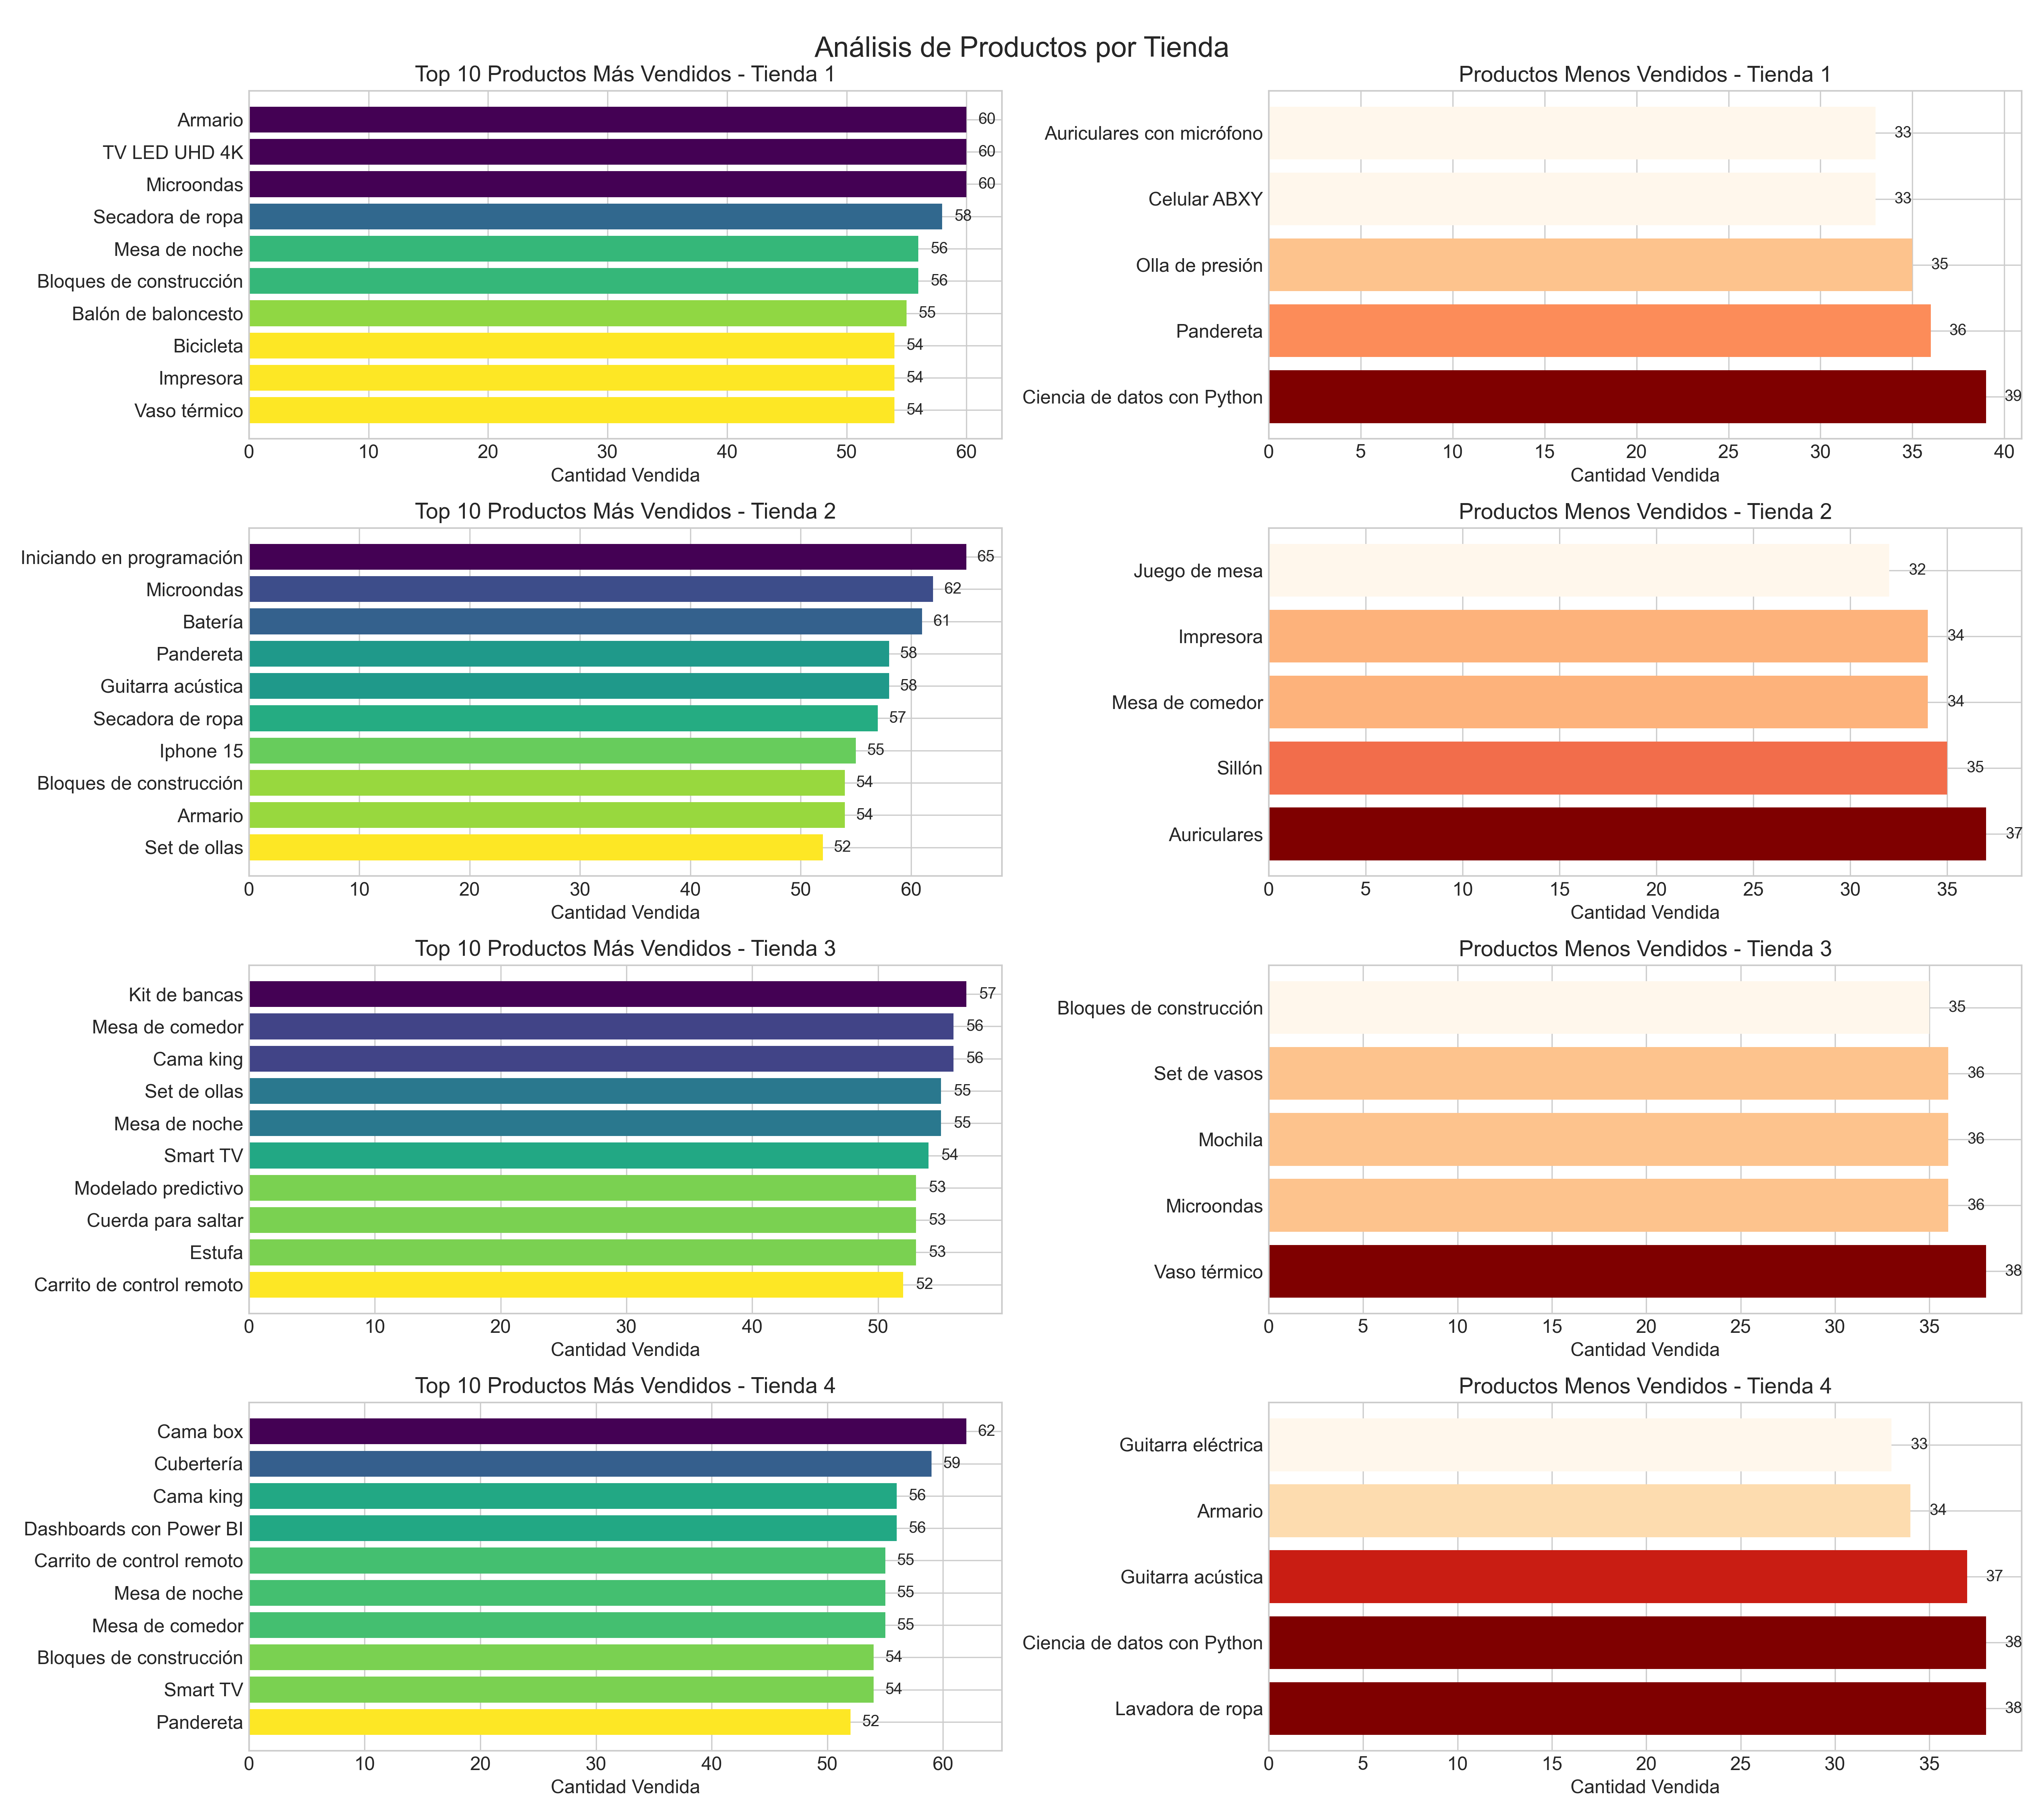
\includegraphics[width=\textwidth]{4_productos_vendidos.png}
\end{center}

El análisis de productos muestra una distribución bastante uniforme de ventas entre tiendas, con algunos productos específicos destacando en cada establecimiento.

\chapter{Análisis de Costos de Envío}

\section{Costo Promedio de Envío por Tienda}

El costo de envío afecta directamente la rentabilidad de cada operación. A continuación se muestra una comparación:

\begin{center}
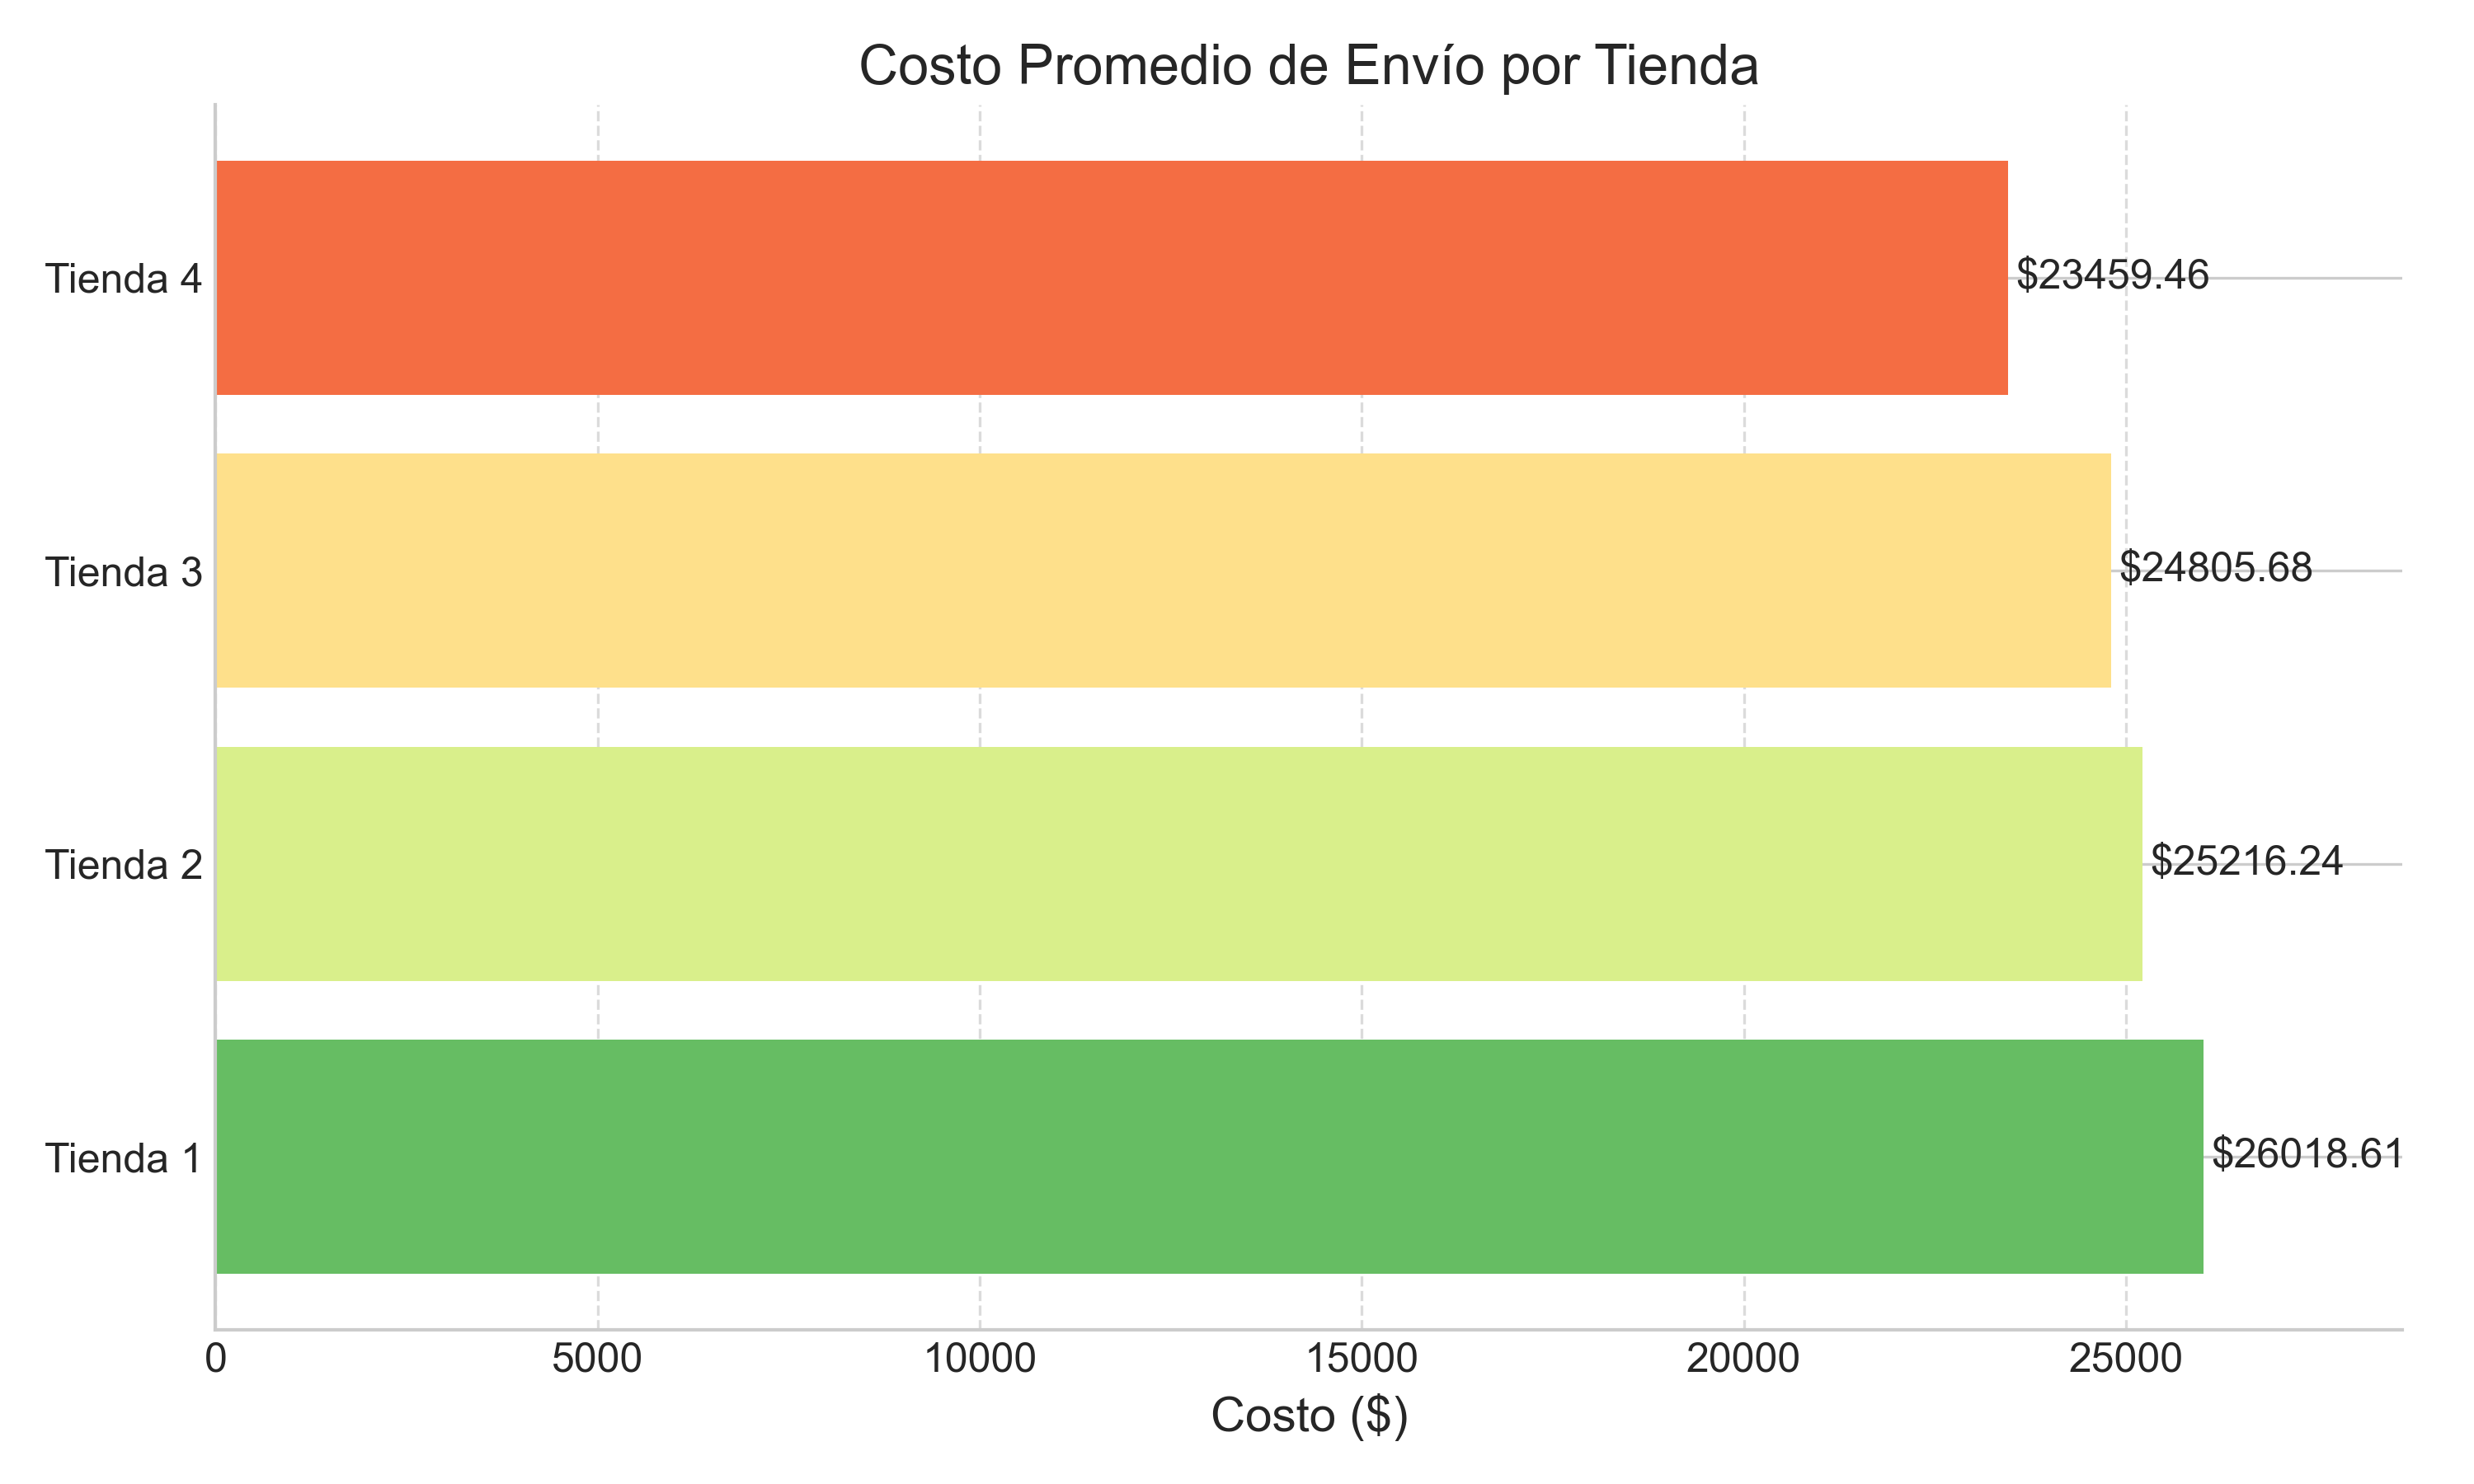
\includegraphics[width=0.8\textwidth]{5_costo_envio.png}
\end{center}

El análisis de costos de envío muestra:

\begin{itemize}
    \item La Tienda 1 tiene el costo promedio de envío más alto (\$26,019).
    \item La Tienda 4 tiene el costo promedio de envío más bajo (\$23,459).
    \item Existe una diferencia de aproximadamente 10\% entre el costo más alto y el más bajo.
    \item Un menor costo de envío es favorable para la rentabilidad, lo que da una ventaja a la Tienda 4 en este aspecto.
\end{itemize}

\chapter{Análisis Comparativo}

\section{Resumen de Indicadores}

Para facilitar la toma de decisiones, se ha creado un análisis comparativo con las métricas normalizadas y ponderadas:

\begin{center}
\begin{tabular}{lccccc}
\toprule
\textbf{Tienda} & \textbf{Facturación} & \textbf{Evaluación} & \textbf{Costo Envío} & \textbf{Ventas} & \textbf{Puntuación} \\
\midrule
Tienda 1 & \$1,150,880,400 & 3.98 & \$26,019 & 2,359 & 0.846 \\
Tienda 2 & \$1,116,343,500 & 4.04 & \$25,216 & 2,359 & 0.843 \\
Tienda 3 & \$1,098,019,600 & 4.05 & \$24,806 & 2,359 & 0.841 \\
Tienda 4 & \$1,038,375,700 & 4.00 & \$23,459 & 2,358 & 0.827 \\
\bottomrule
\end{tabular}
\end{center}

\section{Análisis de Radar}

A continuación se presenta un gráfico de radar que permite visualizar el rendimiento relativo de cada tienda en los diferentes indicadores:

\begin{center}
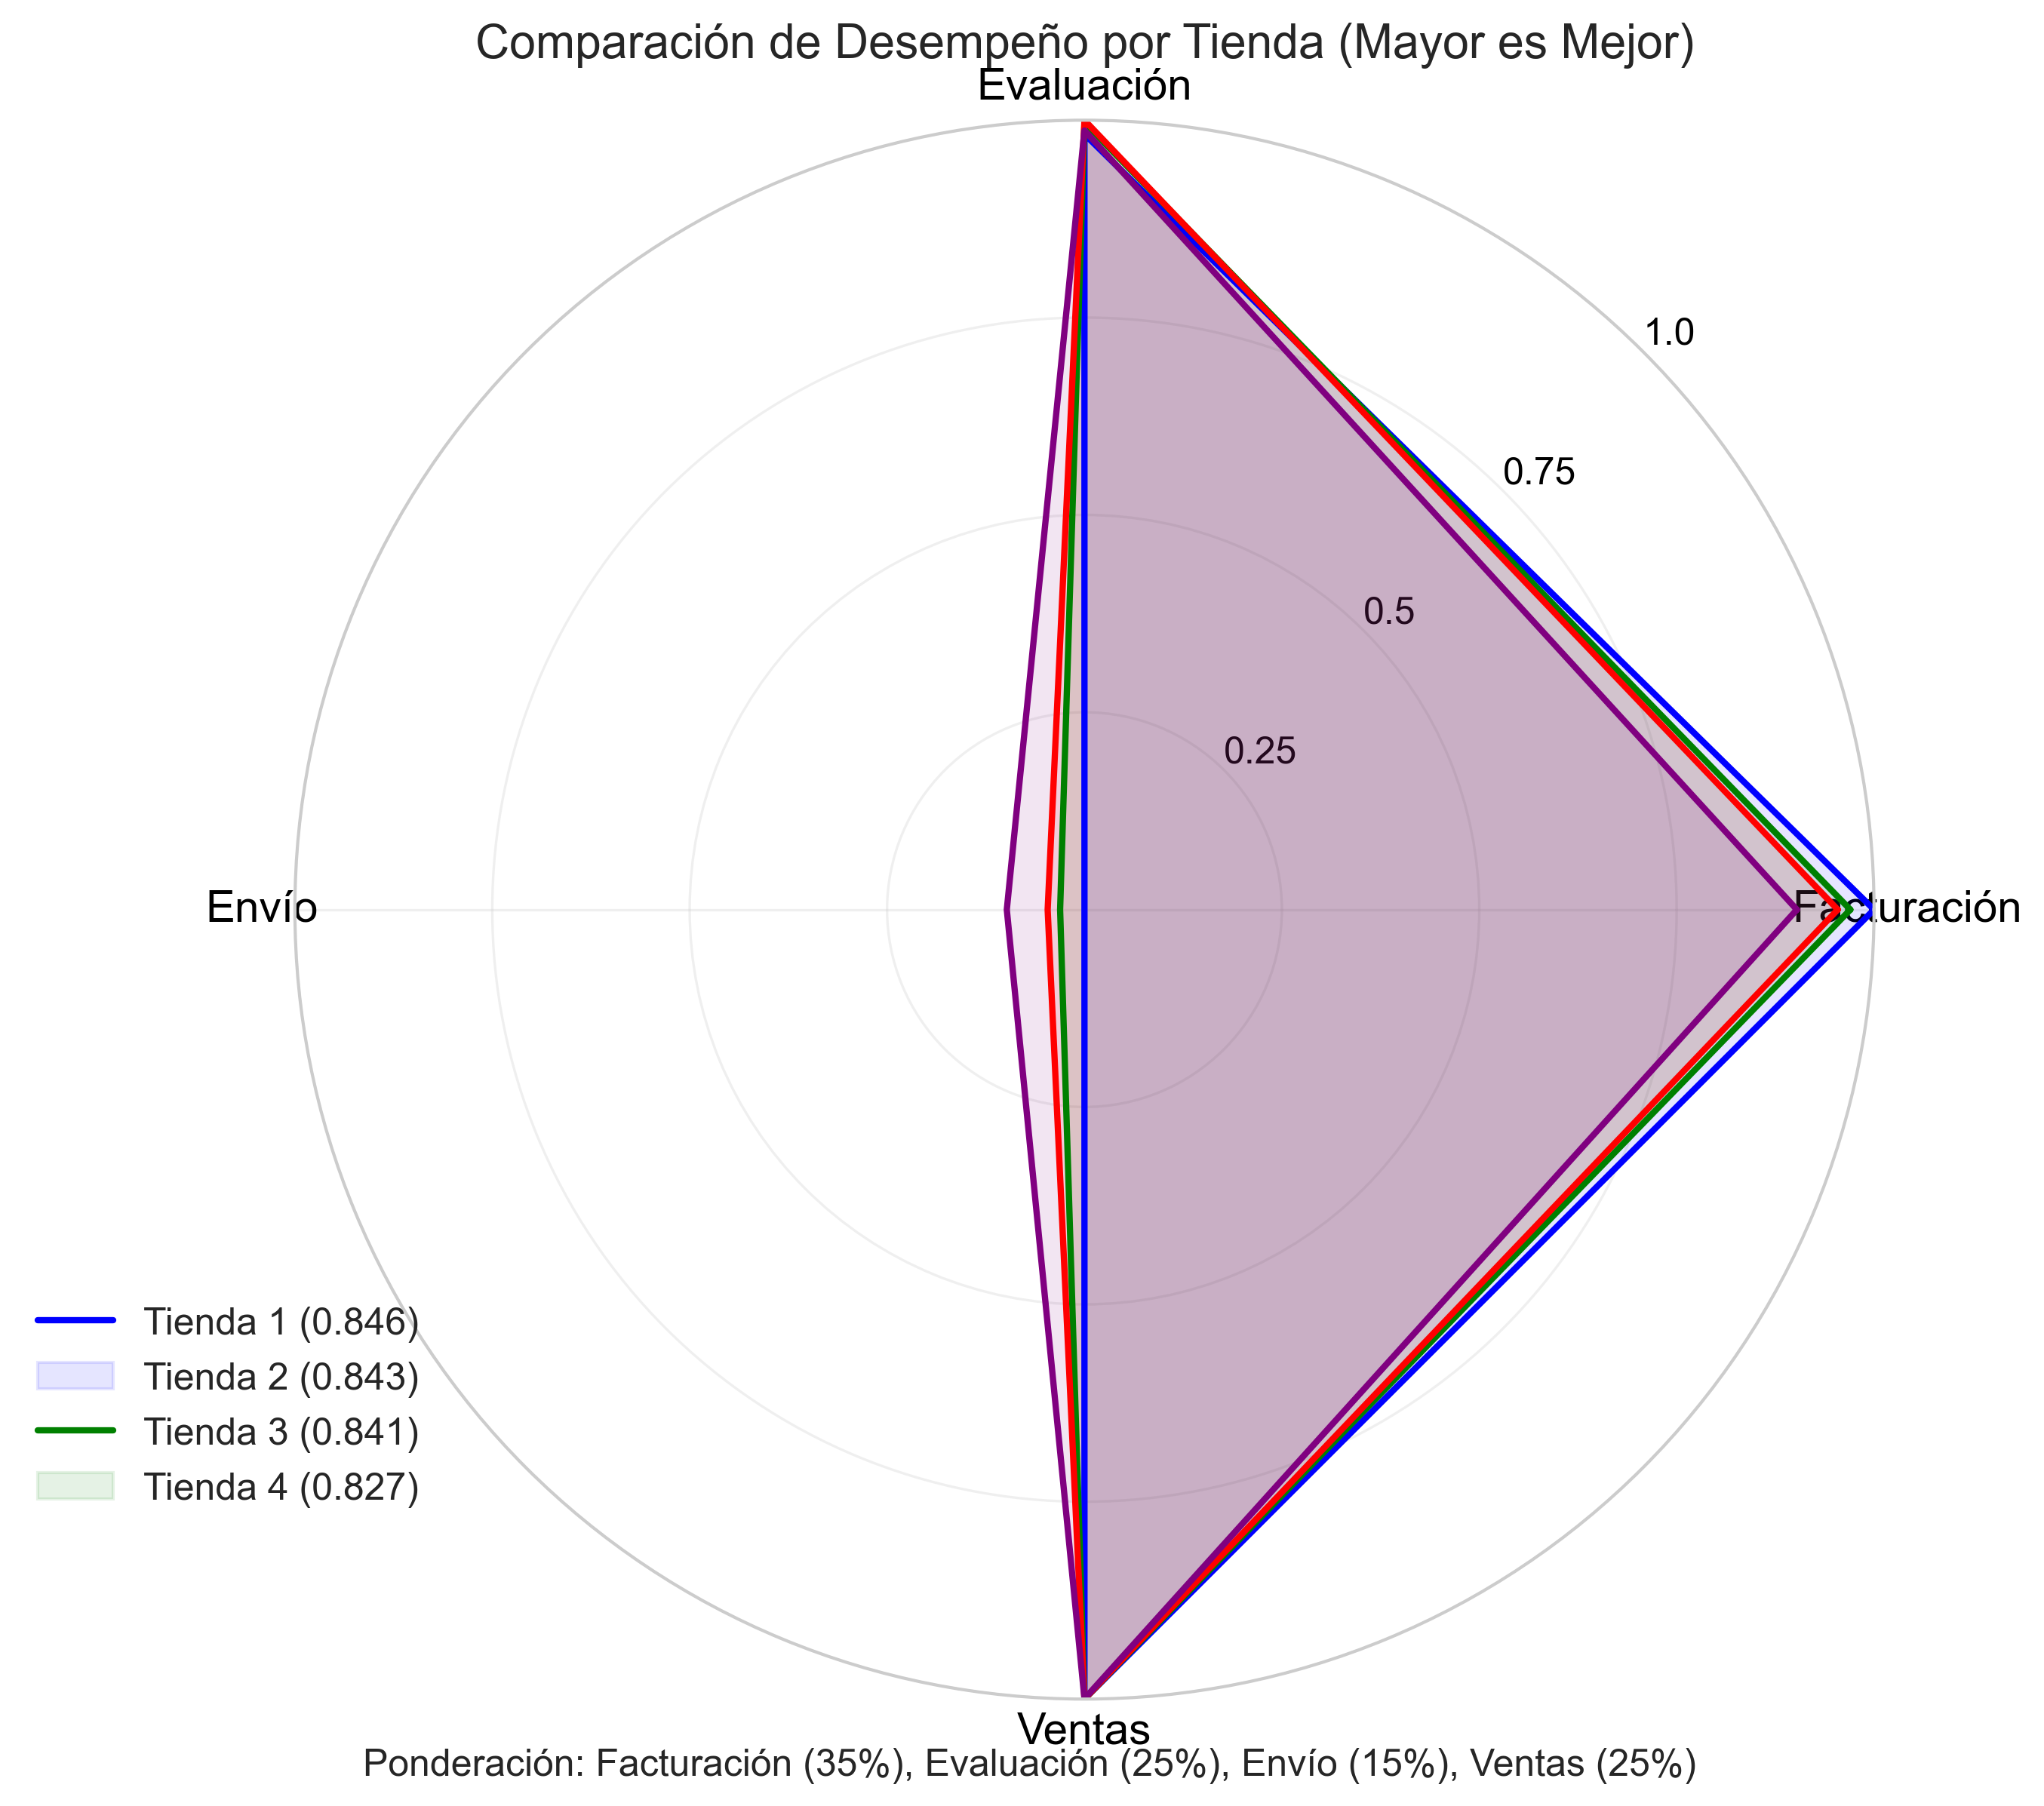
\includegraphics[width=0.8\textwidth]{6_puntuacion_total.png}
\end{center}

\begin{center}
\textbf{Leyenda:} FAC = Facturación, EVA = Evaluación de Clientes, VEN = Volumen de Ventas,\\ 
ENV = Costo de Envío (Normalizado inversamente, mayor valor = menor costo)
\end{center}

\chapter{Recomendación y Conclusiones}

\section{Recomendación Final}

Tras un análisis exhaustivo de los diversos indicadores de desempeño, se recomienda al Sr. Juan vender la \textbf{Tienda 4} por las siguientes razones:

\begin{enumerate}
    \item Presenta la puntuación total más baja (0.827) en el análisis comparativo ponderado.
    \item Tiene la facturación total más baja (\$1,038 millones), aproximadamente un 10\% inferior a la tienda con mayor facturación.
    \item Si bien tiene el costo de envío más favorable, este factor no compensa las desventajas en los otros indicadores más relevantes.
    \item La evaluación de clientes, aunque no es la más baja, se encuentra por debajo de la Tienda 2 y Tienda 3.
\end{enumerate}

\section{Consideraciones Estratégicas}

Es importante destacar que todas las tiendas muestran un desempeño relativamente similar, con diferencias porcentuales pequeñas en varios indicadores. Esto sugiere que cualquiera de las tiendas podría ser una candidata razonable para la venta.

Sin embargo, la Tienda 4 muestra consistentemente un desempeño ligeramente inferior en los indicadores de mayor peso estratégico, como la facturación total y el volumen de ventas, lo que la convierte en la opción más adecuada para vender e invertir esos recursos en un nuevo negocio con mayor potencial de crecimiento.

\section{Próximos Pasos}

Se recomienda al Sr. Juan:

\begin{enumerate}
    \item Iniciar conversaciones con potenciales compradores para la Tienda 4.
    \item Realizar una valoración financiera detallada que incluya activos, pasivos y proyección de flujos futuros.
    \item Desarrollar un plan de transición para minimizar cualquier impacto negativo durante el proceso de venta.
    \item Evaluar oportunidades específicas para el nuevo negocio donde se realizará la inversión.
\end{enumerate}

\end{document} 